%% The first command in your LaTeX source must be the \documentclass command.
%%
%% Options:
%% twocolumn : Two column layout.
%% hf: enable header and footer.
\documentclass[
% twocolumn,
% hf,
]{ceurart}

%%
%% One can fix some overfulls
\sloppy

%%
%% Minted listings support 
%% Need pygment <http://pygments.org/> <http://pypi.python.org/pypi/Pygments>
\usepackage{listings}
\usepackage{subfigure}
%% auto break lines
\lstset{breaklines=true}
\newtheorem{theorem}{Theorem}[section]
\newtheorem{definition}{Definition}[section]
%%
%% end of the preamble, start of the body of the document source.
\begin{document}

%%
%% Rights management information.
%% CC-BY is default license.
\copyrightyear{2022}
\copyrightclause{Copyright for this paper by its authors.
  Use permitted under Creative Commons License Attribution 4.0
  International (CC BY 4.0).}

%%
%% This command is for the conference information
\conference{Woodstock'22: Symposium on the irreproducible science,
  June 07--11, 2022, Woodstock, NY}

%%
%% The "title" command
\title{Neural-Symbolic Predicate Invention: \\Learning Relational Concepts from Visual Scenes}

\tnotemark[1]
\tnotetext[1]{You can use this document as the template for preparing your
  publication. We recommend using the latest version of the ceurart style.}

%%
%% The "author" command and its associated commands are used to define
%% the authors and their affiliations.
\author[1,2]{Dmitry S. Kulyabov}[%
orcid=0000-0002-0877-7063,
email=kulyabov-ds@rudn.ru,
url=https://yamadharma.github.io/,
]
\cormark[1]
\fnmark[1]
\address[1]{Peoples' Friendship University of Russia (RUDN University),
  6 Miklukho-Maklaya St, Moscow, 117198, Russian Federation}
\address[2]{Joint Institute for Nuclear Research,
  6 Joliot-Curie, Dubna, Moscow region, 141980, Russian Federation}

\author[3]{Ilaria Tiddi}[%
orcid=0000-0001-7116-9338,
email=i.tiddi@vu.nl,
url=https://kmitd.github.io/ilaria/,
]
\fnmark[1]
\address[3]{Vrije Universiteit Amsterdam, De Boelelaan 1105, 1081 HV Amsterdam, The Netherlands}

\author[4]{Manfred Jeusfeld}[%
orcid=0000-0002-9421-8566,
email=Manfred.Jeusfeld@acm.org,
url=http://conceptbase.sourceforge.net/mjf/,
]
\fnmark[1]
\address[4]{University of Skövde, Högskolevägen 1, 541 28 Skövde, Sweden}

%% Footnotes
\cortext[1]{Corresponding author.}
\fntext[1]{These authors contributed equally.}

%%
%% The abstract is a short summary of the work to be presented in the
%% article.
\begin{abstract}
The predicates used for Inductive Logic Programming (ILP) systems are typically elusive and need to be hand-crafted in advance limiting the generalization of the system when learning new rules without sufficient background knowledge. Predicate Invention (PI) for ILP is the problem of discovering new concepts that describe hidden relationships in the domain. PI can mitigate the generalization problem by inferring new concepts such that the system gains better vocabularies to compose logic rules to solve problems. Although several PI approaches for symbolic ILP systems exist, PI for NeSy ILP systems, which can deal with visual inputs to learn logic rules using differentiable reasoning, is relatively unaddressed. To this end, we propose a neural-symbolic approach to invent predicates from visual scenes for NeSy ILP systems based on clustering and extension of relational concepts. Our NeSy PI model handles visual scenes as its input using deep neural networks for the visual perception, and invents new concepts which are useful to solve the task of classifying complex visual scenes. The invented concepts can be used by NeSy ILP systems instead of hand-crafted background knowledge. Our experiments show that the PI model is capable of inventing high-level concepts and solving complex visual logical patterns. Moreover, the invented concepts are explainable and interpretable while also providing competitive results with the state of the art NeSy ILP systems with given knowledge.
\end{abstract}

%%
%% Keywords. The author(s) should pick words that accurately describe
%% the work being presented. Separate the keywords with commas.
\begin{keywords}
	Predicate Invention \sep
	Inductive Logic Programming \sep
	Neural Symbolic Artificial Intelligence\sep
\end{keywords}

%%
%% This command processes the author and affiliation and title
%% information and builds the first part of the formatted document.
\maketitle

\section{Introduction}


Neural Symbolic Inductive Logical Programming (NeSy-ILP) learns logical programs from images. 
Such learned program sences the inherent logic in the Visual Scenes and consider them as rules for classification task.  An example of such patterns is shown in figure \ref{fig:intro-hide}. In order to solve such patterns, a set of predicates are required, for example $\mathtt{blue\_sphere} $ defines the existence of a sphere with color blue. 

However, to describe logical relations, these predicates in NeSy-ILP systems are either given as pretrained neural predicates or as hand-crafted background knowledge. 
If any background knowledge or predicates are incorrect or unprovided, the optimal program searching can be failed. Thus it is essential for system to conquer the problem of depending of given knowledge but generate new language by itself. Besides, background knowledge can be hard to collect and usually provided by human experts, which limits the applying domain of ILP systems.

Predicate invention(PI)\cite{pi1988} is one direction to solve this problem, which is also a sub-problem in ILP. It works for ILP system to invent new predicates as symbols for new concepts based on well designed basic predicates, which enlarge the expression of the language in ILP. In our example, the concept $ \mathtt{blue\_sphere} $ is given as BK knowledge, but with PI system, such concepts are learned from separate basic concepts $ \mathtt{blue} $ and $ \mathtt{sphere} $. However, most ILP system doesn't support PI, since it is hard to define when and how to generate new predicates. 

%% Tell some reasons if possible

\begin{figure*}[h]
	\centering
	\begin{minipage}{0.4\textwidth}
		\centering
		
\includegraphics[width=0.3\linewidth]{img/intro_hide/true1.png} 
		
\includegraphics[width=0.3\linewidth]{img/intro_hide/true2.png} 
		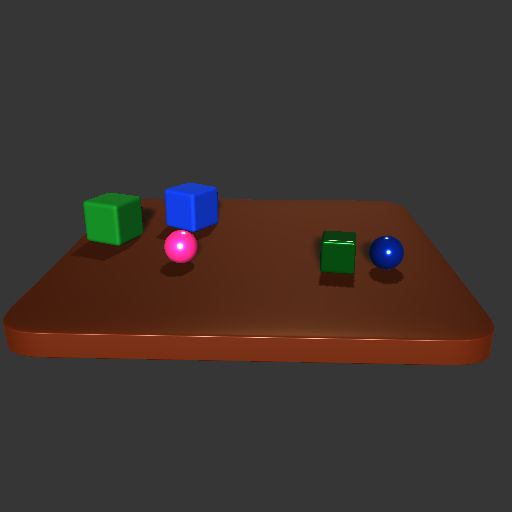
\includegraphics[width=0.3\linewidth]{img/intro_hide/true3.png} 
		
		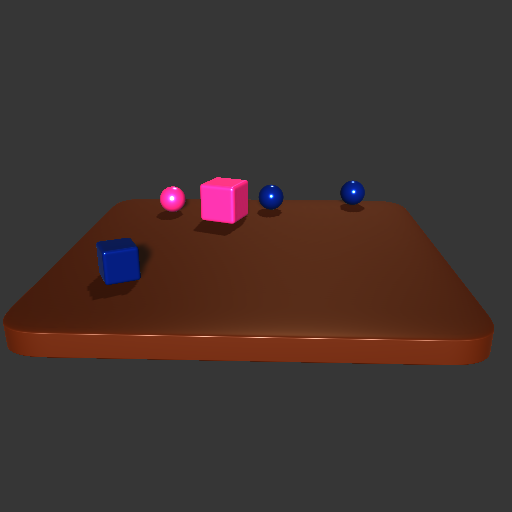
\includegraphics[width=0.3\linewidth]{img/intro_hide/false1.png} 
		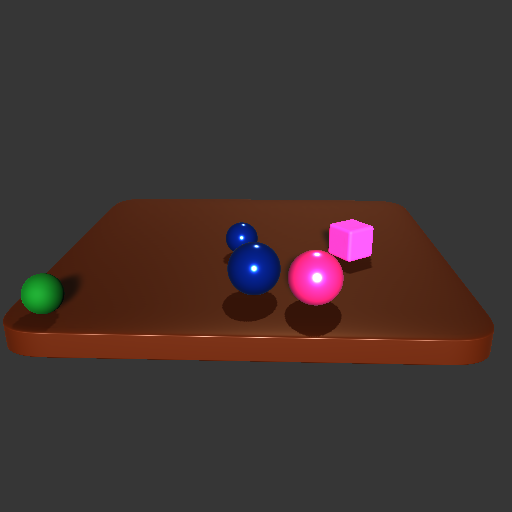
\includegraphics[width=0.3\linewidth]{img/intro_hide/false2.png}
		
\includegraphics[width=0.3\linewidth]{img/intro_hide/false3.png}
		\label{fig:intro-hide}
		\end{minipage}
		\begin{minipage}{0.55\textwidth}
			\centering
			
\includegraphics[width=\linewidth]{img/intro_hide/intro_bk.png} 
			\label{fig:intro-bk}
		\end{minipage}
			\caption{A logic Pattern in 3D scenes can be learned by Neural-Symbolic ILP system. Positive images on the first row, negative images on the second row. The truth pattern is: a blue sphere either locate on the left side of a green sphere or locate on the right side of a green cube.}
\end{figure*}

Either placed on the side 


We propose a neural-symbolic PI approach based on \textit{clustering} and \textit{extension} of relational concepts, which is able to reasoning visual scenes without background knowledge. The knowledge can be summarized from scenes. It evaluates the clauses based on its characteristics of necessity and sufficiency. The procedure is repeated iteration by iteration, until the target clauses are found. We tested our approach on both 2D and 3D image patterns.

Comparing to existing approaches, our approach has following contributions

\begin{itemize}
	\item We proposed a predicate invention approach for neural symbolic ILP system.
	\item A formalized way to efficiently evaluate the clauses in visual scenes, which can be further used for pruning.
	\item We discussed about \textit{when} and \textit{how} to invent new predicates based on \textit{necessary} and \textit{sufficient} judgment factors.
	\item The implementation.
	
\end{itemize}





\section{Background and Related Work}

Although predicate invention has been proposed since 1988 by \cite{MUGGLETON1988339}, it is always be considered as a major challenge. Most ILP system do not supports PI, including classic systems like Progol \cite{Muggleton1995InverseEA}, TILDE\cite{BLOCKEEL1998285} and modern system such as ATOM \cite{atom}, LFIT \cite{LFIT}.

Some works have been proposed for PI systems. However, none of these are focus on visual images and learning logical patterns existing in the visual scenes. 
\cite{pilff} is an approach for predicate invention, which generate constrains from inconsistent hypothesis and further be used for pruning all the similar clauses. \cite{gtnpi} use negation with PI to generalize the clause, which follows a bottom-top direction 
Several system uses \cite{Evans2018}, \cite{kaminski_eiter_inoue_2018} meta-rules as templates for new predicates invention. 

$ \alpha $ILP (citation?) supports visual image as input but require background knowledge during the reasoning.


 
 

\section{Target Map}

Collect the facts from group of visual scenes and induce the common properties from the facts are 
can answer the question, why they are in the same group. However, common properties sometimes can be not obviously and hard to be described.
and using a single word  to summarize it to a suitable new concept is one of powerful ability of human-being. It simplifies the description of complex 
Predicate invention is an essential ability for ILP system to reasoning about 

\begin{figure*}[h]
	\centering
	\begin{minipage}{\textwidth}
		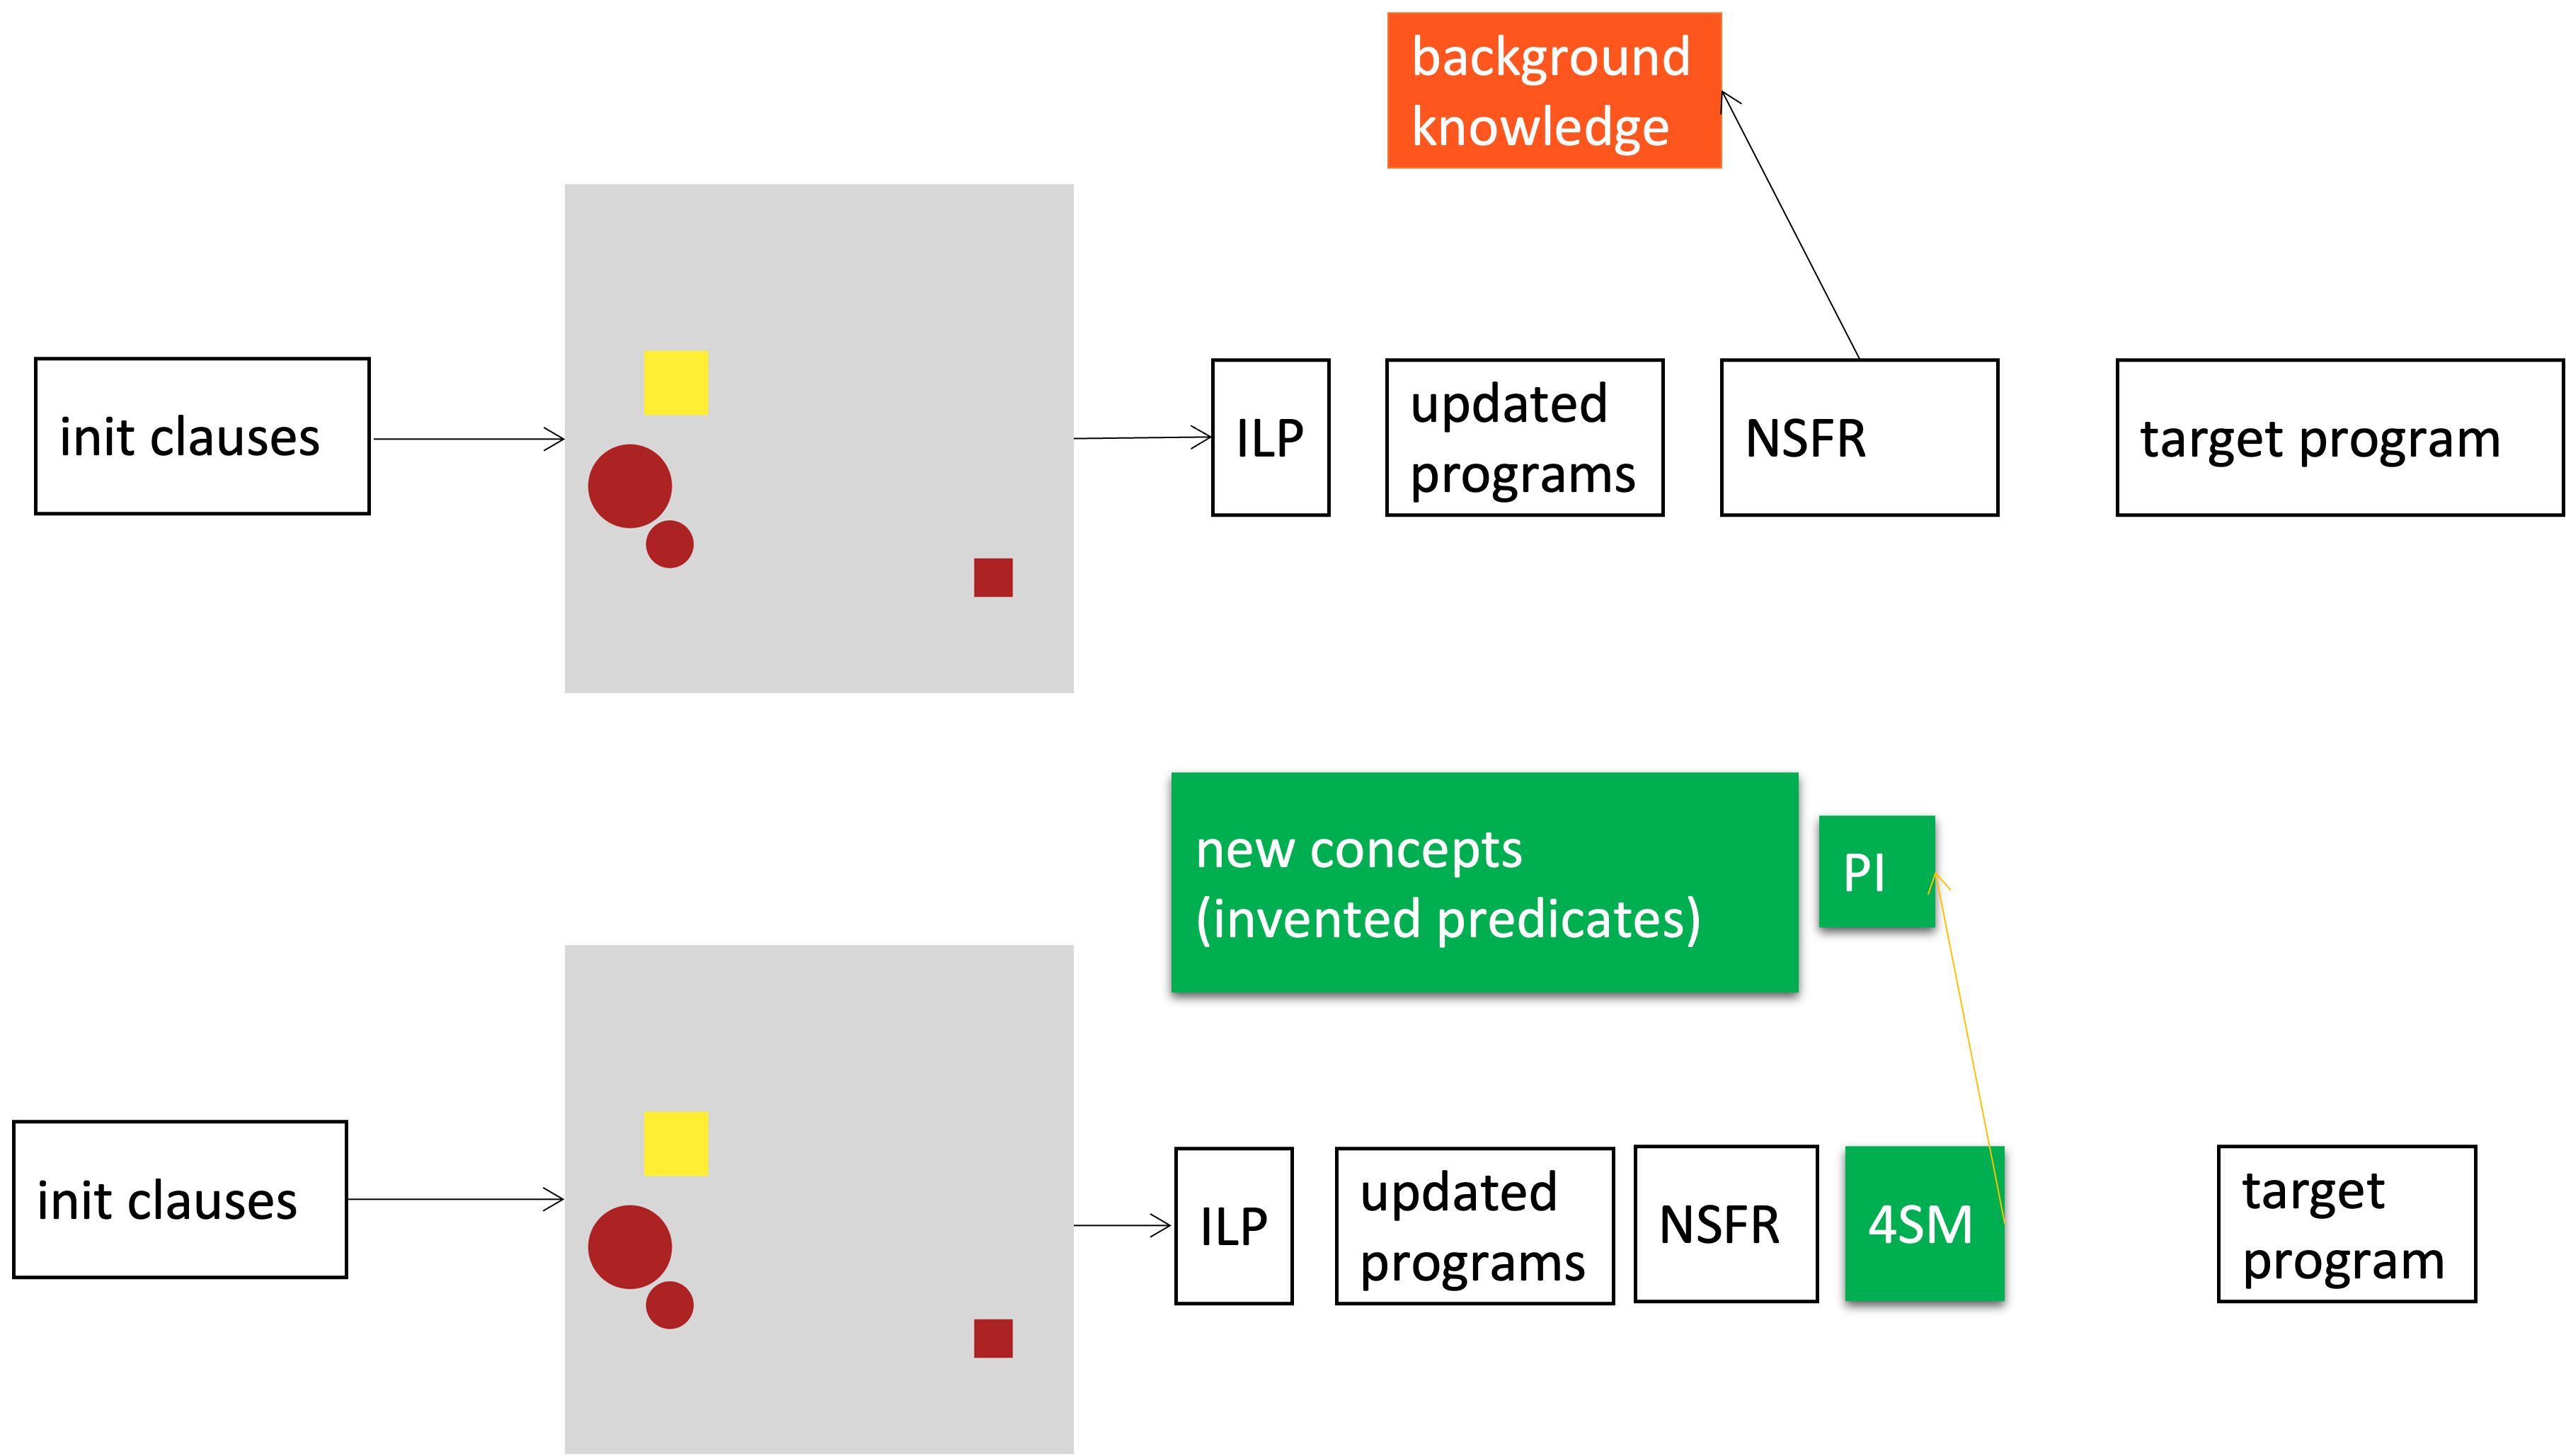
\includegraphics[width=\linewidth]{img/intro_compare.png} 
		\caption{Predicate invention workflow.}
		\label{fig:Pipeline comparison between neural symbolic-ILP system without PI module and with PI module.}
	\end{minipage}
\end{figure*}


\begin{figure*}[h]
	\centering
	\begin{minipage}{\textwidth}
		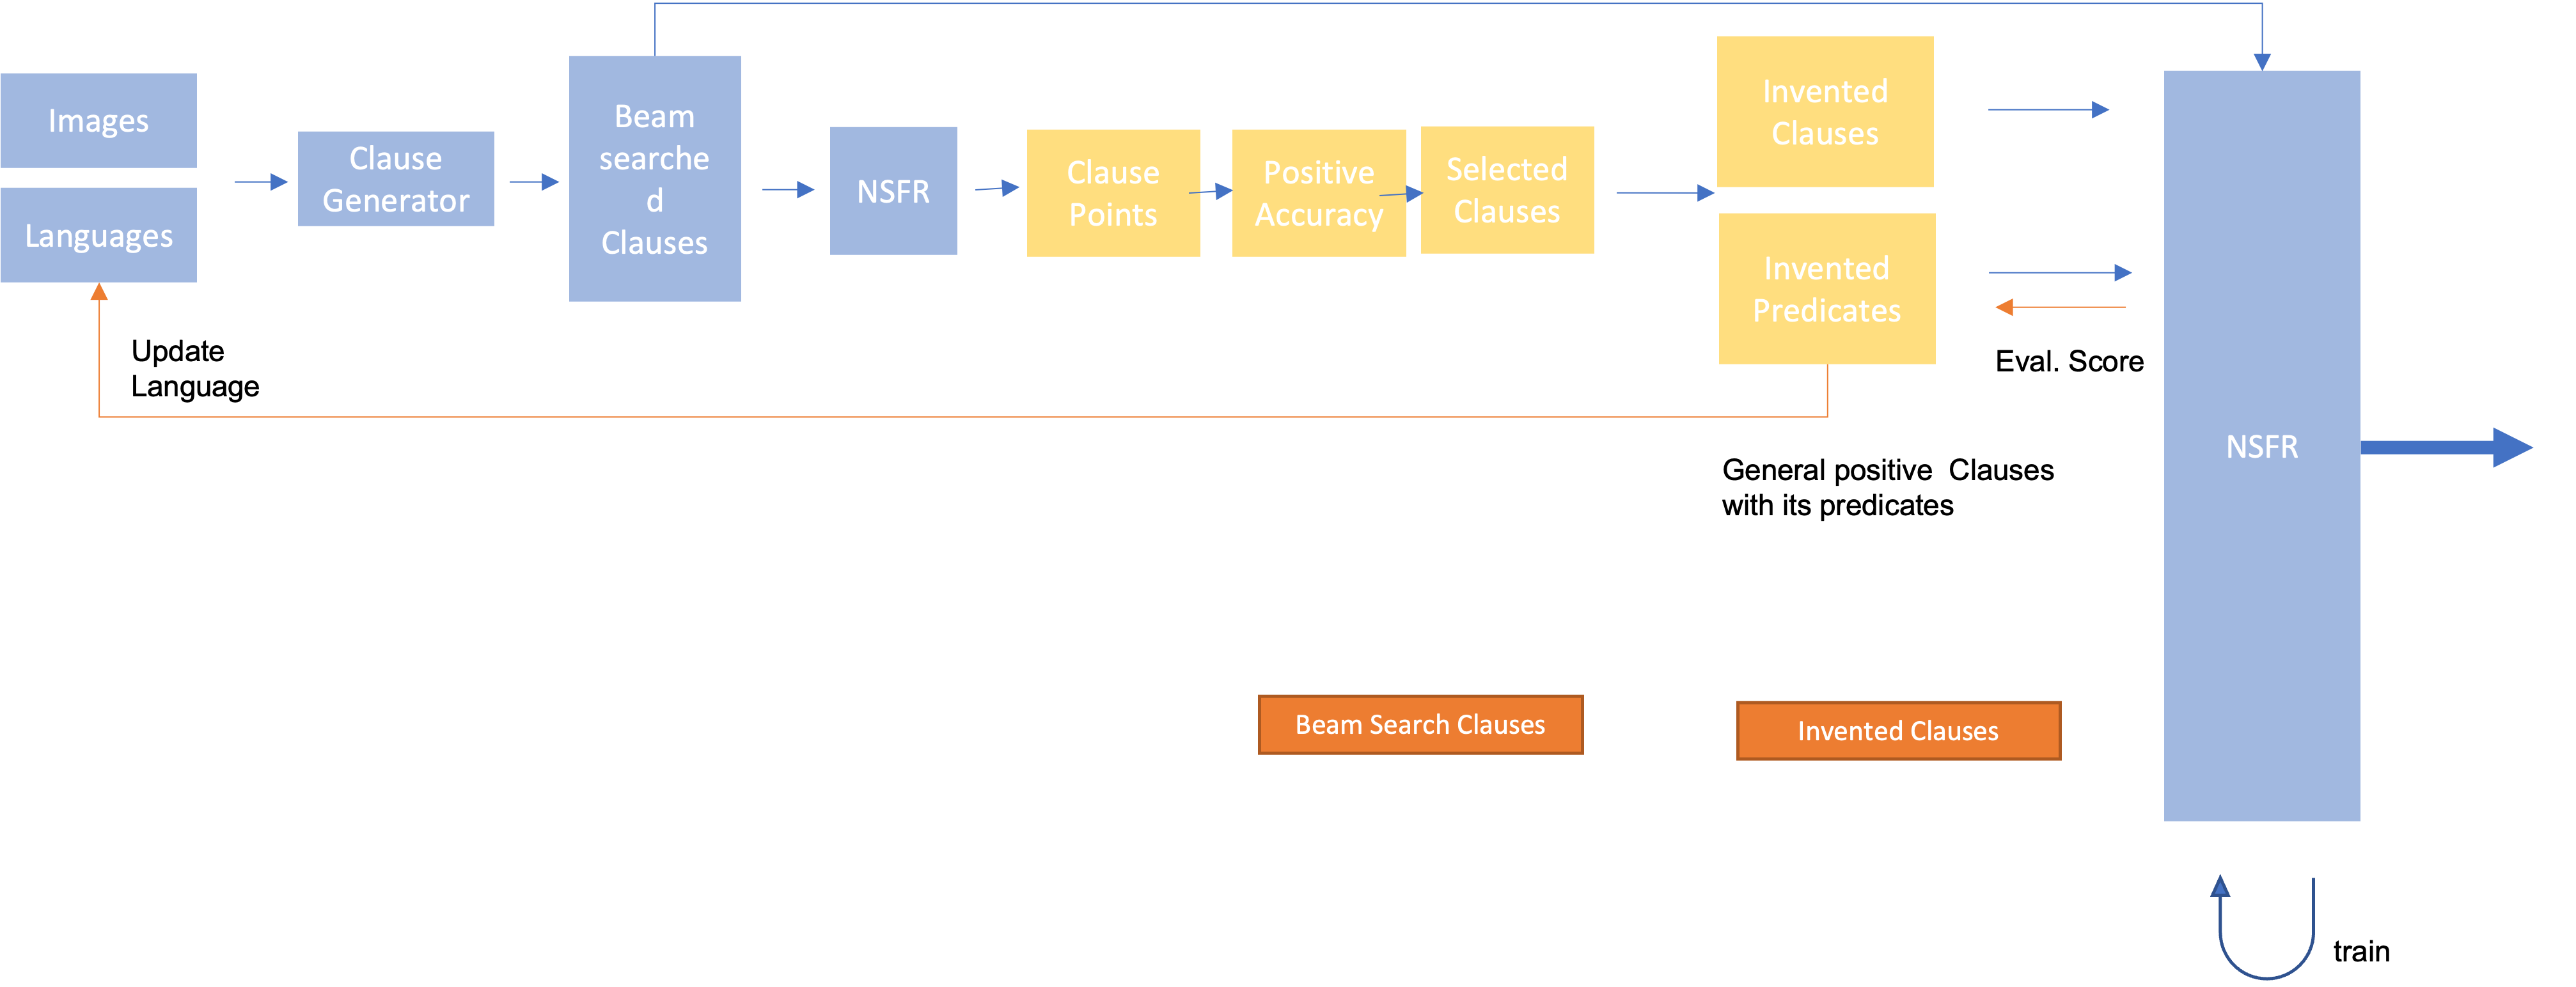
\includegraphics[width=\linewidth]{img/pi_structure.png} 
		\caption{Predicate invention workflow.}
		\label{fig:pi-structure}
	\end{minipage}
\end{figure*}

The goal of our work is to find a predicate invention pipeline so that some high level concepts are not necessarily given from reasoning language directly. But they can be invented as needed during training. The invention is important since it is a way to acquire new knowledge and shows the ability of intelligence. On the other hand, it improves the generalization of AI models for adapting unseen tasks. The invention model improves the system to describe the problem more accurate.

%TODO: rewrite...
However, the invention is still based on given background knowledge. It has to be simple, combinable,  and mutually compatible, so that the new concepts are various and accurate.

In order to using a single language to cover two objects spatial relations as many as possible, we designed an area division map called \textit{target map}. As shown in figure \ref{fig:8-area}, the surrounding area according to the reference object has been divided into 8 sub-areas. 
The areas in the target map are considered as background knowledge. The concepts like left, right, nearby supposed to be invented as new predicates during the training if any of them are needed to represent the target pattern in the positive images.  This map both considers the distance and directions of the latent relation objects. 
Using the target map, multiple real-world related spatial concepts can be represented by combining some of atom areas, such as 
\textit{left} (combining area 2,3,6,7), 
\textit{right}(combining area 0,1,4,5), 
\textit{nearby}(combining area 0,1,2,3) and so on. 

\newpage
\section{Predicate Invention}


The target of inductive logic programming is to find a target clause $ P $ for the positive patterns $ Q $ , such that the clause $ P $ describes some logical relations that exist and only exist in the positive patterns. 
Thus the target clause $ P $ is sufficient and necessary for the positive patterns $ Q $.
\[ P\Leftrightarrow Q \]


\begin{definition}[PN pair]
	A pair of positive and negative images.
\end{definition}
%TODO: tell the way of clause generation
We prepare equal number of positive and negative images for evaluation, thus all the images can be paired from two groups.
A new generated clause is evaluated on all the PN pairs. Evaluation on each pair getting two values, one from positive and one from negative. 
 We can take negative value as x axis, positive value as y axis and draw all the evaluation result on a coordinate system. Thus each PN pair corresponds a point. We observed these points are only appears in the four clusters in the coordinate system( as show in figure \ref{fig:mce-example} left.), thus we fuzzy these points to only four areas (we use $ f(P) $ to represent this step, where $ P $ is the points on the whole dataset.), each take one cluster. Thus for these two values, we only have $ 2^2=4 $ different combinations. We named it as \textit{four score map}.  
 
 \begin{figure*}[h]
 	\centering
 	\begin{minipage}{\textwidth}
 		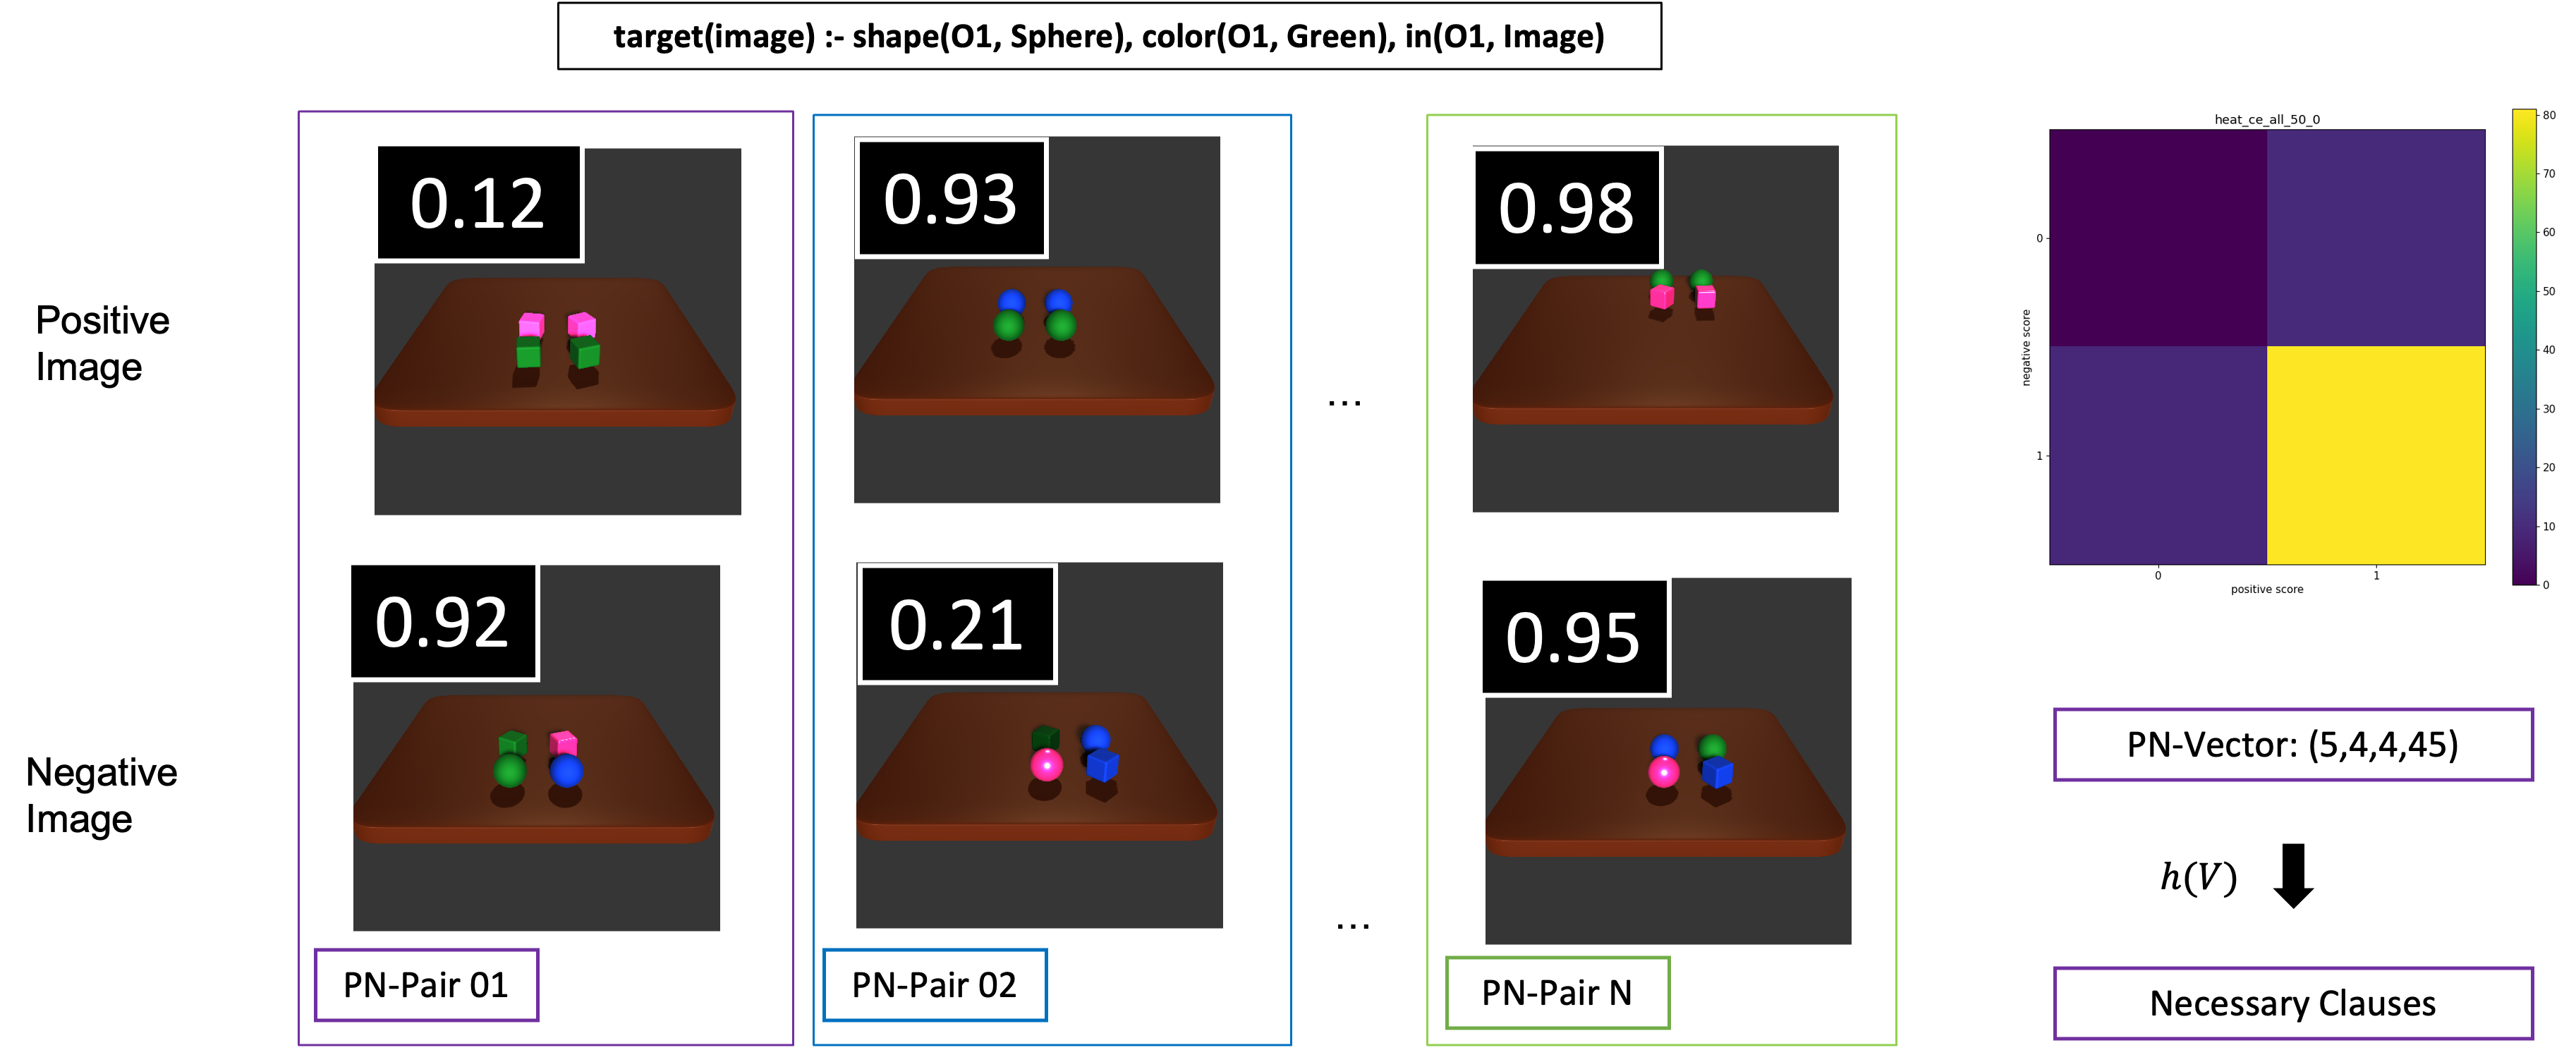
\includegraphics[width=\linewidth]{img/four_zone_explain.png} 
 		\caption{\textbf{Left}: PN pairs. \textbf{Middle}: PN pair scores on coordinate system. The points are clustered in four corners. These scores are evaluated by NSFR. \textbf{Right:}Four Score Map. The four score map illustrates the result of 4 kinds of evaluation on one clause, i.e. high positive-high negative, high positive-low negative, low positive-high negative, low positive-low negative. }
 		\label{fig:pn-pair}
 	\end{minipage}
 \end{figure*}
 
 A \textbf{four score map} fuzzy the evaluation result on an image to positive 1 and negative 0, map the positive image result and negative image result to four areas, namely $ (0,0), (0,1), (1,0) $ and $ (1,1) $. We found that four score map has good description for sufficient and necessary conditions in logic.

Base on the scoring areas of the predicates, we can classify them into several groups. Let $ N $ denotes the number of PN pairs.

\begin{definition}[Sufficient and Necessary Clause]
	Scores on $ (0,1) $ only, i.e. $ s_{01} =N$ They are sufficient and necessary for the target pattern.
\end{definition}

\begin{definition}[Necessary Clause]
	Scores on $ (0,1) $ and $ (1,1) $, i.e. $ s_{01} + s_{11} = N $. They are necessary for the target pattern. Note that they always true in the positive images, but also can be true in negative images.
\end{definition}

\begin{definition}[Sufficient Clause]
	Scores on $ (0,0) $ and $ (0,1) $, $ s_{00}+s_{01} = N $ and $ s_{01}>0 $. It induces directly some of positive patterns but can be failed on some other positive patterns. It never induces any negative patterns.
\end{definition}

The key idea of these definitions is to find a way to provide promising clauses for extension or clustering. Since it is impossible to extended every clauses and check its score, or try to cluster any number of existing clauses. Thus a prune strategy is required for promising clause generation. We consider necessary clauses and sufficient clauses as promising clauses. For each iteration of clause generation, we extend only these two kinds of clauses, which can significantly reduce the number of new clauses, whereas the rest clauses are pruned. In the PI section, the new predicates are acquired by clustering of same type of clauses, i.e. they are either clustered from necessary clauses only or from sufficient clauses only.




\subsection{Clause Generation by Extension}
We getting new clauses by extend the existing clauses with knowing predicates in the language. In every experiment, the clause extension starting from the most general one, i.e. $ \mathtt{target(X):-in(O1,X),in(O2,X).} $, whereas the number of predicate $ in(O,X) $ depends on the related object number in the ground truth pattern. Assume there are $ 10 $ predicates exist in the language, to extend one predicate from initial clause can acquire 10 new clauses, to extend 2 predicates can acquire $ 10^2=100 $, and so on. For complicate patterns, the target clauses can require more than 5 predicates or more, thus a prune strategy is necessary during clause extension. We select the clauses those are either necessary or sufficient, which can significantly reduce the number of new clauses after extension.
\begin{align*}
	\mathtt{intermediate\_clause(Tree,Road)&:-left(Tree,Road)} 	\\
\end{align*}

\subsection{Predicate Invention by Clustering}
New predicate invention happens after new clause generation. We acquire new predicates by clustering necessary clauses or sufficient clauses. The new predicates take clustered clauses as their bodies, where clauses in the cluster are considered with $ or $ relation. Clustering can take rules with sub-independent cases into account. For example, a tree placed either on the left side of the road or on the right side of the road can be represented by following predicates

\begin{align*}
	\mathtt{inv\_pred(Tree,Road)&:-left(Tree,Road)} 	\\
	\mathtt{inv\_pred(Tree,Road)&:-right(Tree, Road)}
\end{align*}
To evaluate new predicates, we extent the initial clause with new predicates and evaluate them by four score map. If the new clause is necessary or  sufficient, the corresponding predicate is kept, otherwise it is pruned.





\section{Experiments}
To solve Kandinsky patterns, we provide following constants as background knowledge, 
shape: circle, square, triangle; color: red, yellow, blue; group\_shape: line, unknown; distance: every 25 pixels as one unit. Besides, no further information is given, such as different color, different shape, etc. Some of the patterns are shown in figure \ref{fig:kandinsky-patterns}.

\begin{figure}[!htb]
	\centering
	\subfigure[Nearby]{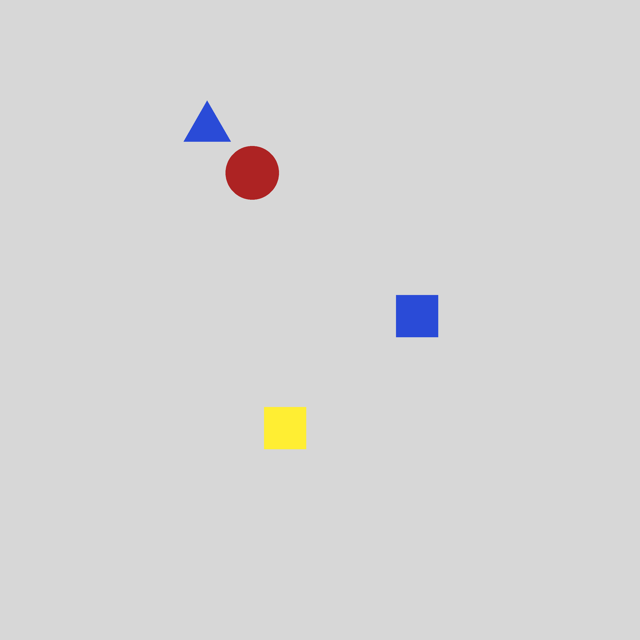
\includegraphics[width=0.24\textwidth]{img/kp/nearby.png}} 
	\subfigure[Two pairs]{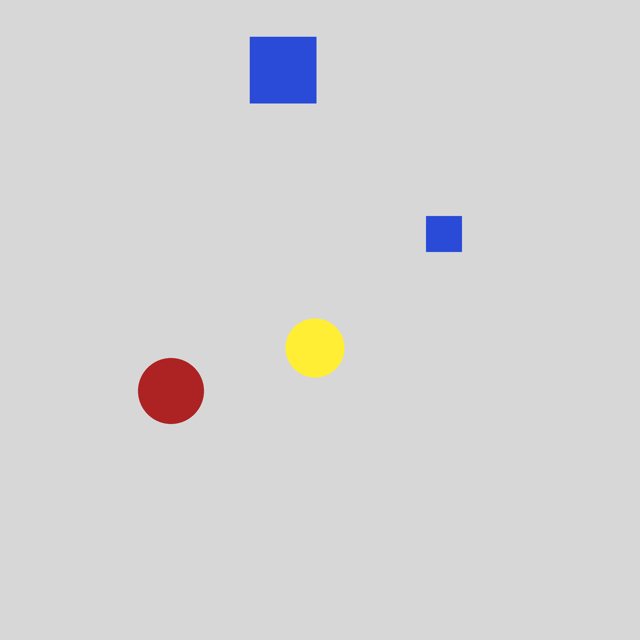
\includegraphics[width=0.24\textwidth]{img/kp/twopairs.png}} 
	\subfigure[Red Triangle]{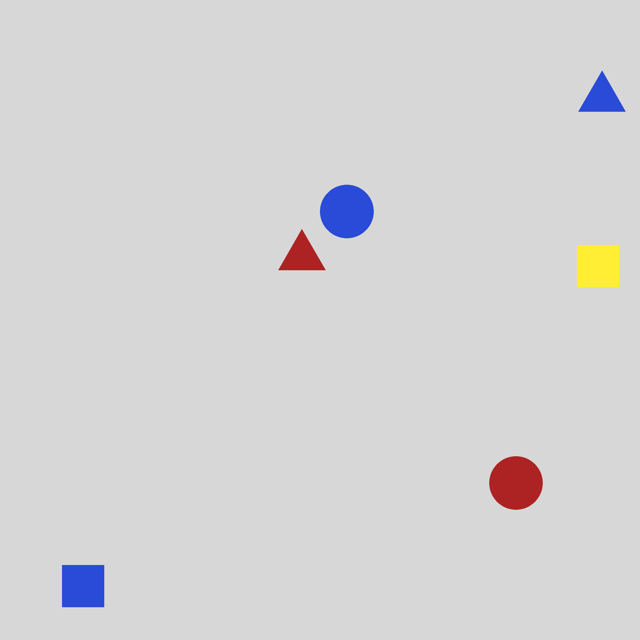
\includegraphics[width=0.24\textwidth]{img/kp/red_triangle.png}} 
	\subfigure[5 Objects Online ]{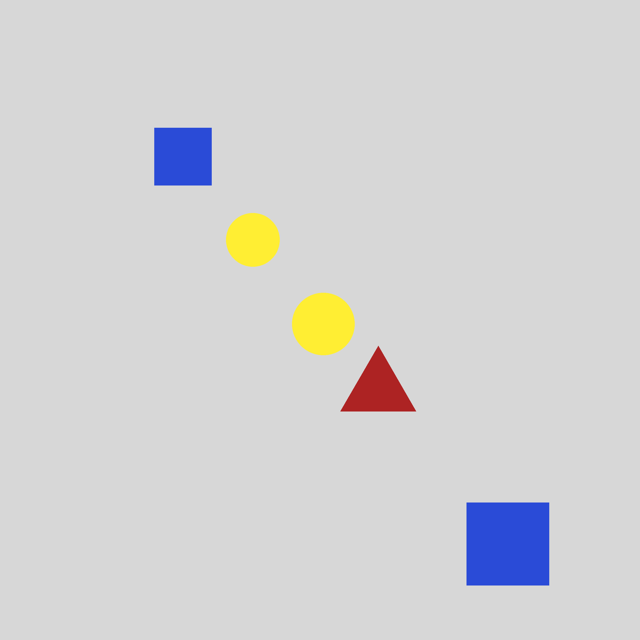
\includegraphics[width=0.24\textwidth]{img/kp/online_pair.png}}
	\caption{Kandinsky Patterns.}
	\label{fig:kandinsky-patterns}
\end{figure}


Learning result of red-triangle pattern is shown as follows:

\begin{lstlisting}[language=Prolog, mathescape]
	target(X):-in(O1,X),in(O2,X),inv_pred25(O1,O2).
	inv_pred0(O1,O2):-in(O1,X),in(O2,X),rho(O1,O2,rho2),shape(O1,circle).
	inv_pred0(O1,O2):-in(O1,X),in(O2,X),rho(O1,O2,rho2),shape(O1,square).
	inv_pred25(O1,O2):-color(O1,red),color(O2,blue),in(O1,X),in(O2,X),inv_pred0(O2,O1),shape(O1,triangle).
	inv_pred25(O1,O2):-color(O1,red),color(O2,yellow),in(O1,X),in(O2,X),inv_pred0(O2,O1),shape(O1,triangle).
	inv_pred25(O1,O2):-color(O1,red),color(O2,yellow),in(O1,X),in(O2,X),inv_pred0(O2,O1),shape(O2,circle).
\end{lstlisting}\\



The performance on each patterns in Kandinsky pattern is shown as follows:
\begin{table}
	\caption{PI Evaluation Result}
	\label{tab:nearby-pi-result}
	\begin{tabular}{ccccc}
		\toprule
		Module              & Nearby & Red-Triangle & Two Pairs & Online\\
		\midrule
		$\alpha$ILP 	    & 1.0 	    & 		    & 		    &           \\
		$\alpha$ILP + PI    & 	1.0 	& 1.0	& 1.0	    &  1.0    \\
		\bottomrule
	\end{tabular}
\end{table}



\begin{table}
	\caption{PI requirement and result on each patterns, where Ne-Preds means neural predicates.}
	\label{tab:pi-result}
	\begin{tabular}{ccccc}
		\toprule
		Patterns             & BK & BK-Clause & \# of Ne-Preds & Completely Learned\\
		\midrule
		red-triangle 	    & 0 	    & 	0	    &  4   &   yes        \\
		two-pairs    & 	0 	& 0	& 3	    &  yes    \\
		5-obj-online    & 	0 	& 0	&  	 1   &   yes   \\
		\bottomrule
	\end{tabular}
\end{table}



\section{Conclusion}

In this paper, we proposed an approach for Neural-Symbolic Predicate Invention. NeSy-PI is able to find the new knowledge and summarize it as new predicates, thus it requires less background knowledge for reasoning.
In our experiment, we show that our PI model can successfully find the target program given only basic neural perception results and relevant constants, no further background knowledge is required. We also show our efficient prune strategy for predicate searching, the searching result is acquired faster and still sound.






To solve the nearby pattern, we invent the concept $ inv\_pred\_1O\_1, O\_2 $ by cluster clauses, which actually represent the concept \textit{nearby}. It is necessary for the target patterns since it is true in all the positive images. It is also directly a sufficient predicate since no negative image has this pattern. The target clauses can be described as follows:
\begin{align*}
	target(X) :- & in(O_1,X),in(O_2,X), inv\_pred\_1(O_1,O_2).\\
	inv\_pred\_1(O_1, O_2) :- 	& in(O_1,X), in(O_2,X), a\_0(O_1,O_2).\\
	inv\_pred\_1(O_1, O_2) :- 	& in(O_1,X), in(O_2,X), a\_1(O_1,O_2).\\									
\end{align*}

\subsubsection{Red Triangle}
To solve the red triangle pattern, we require the concept \textit{nearby} first by cluster clauses. It is necessary for the target patterns but not yet sufficient. Then we use beam search to extend this necessary clause with adding predicates, a sufficient and necessary clause is generated in several steps.
\begin{align*}
	target(X) :- & in(O_1,X),in(O_2,X), inv\_pred\_1(O_1,O_2), \\
						& shape(O_1, triangle), color(O_1, red), \\
						& diff\_shape\_pair(O_1,O_2), diff\_color\_pair(O_1,O_2)\\
	\\
	inv\_pred\_1(O_1, O_2) :- 	& in(O_1,X), in(O_2,X), a\_0(O_1,O_2).\\
	inv\_pred\_1(O_1, O_2) :- 	& in(O_1,X), in(O_2,X), a\_1(O_1,O_2).\\		
	inv\_pred\_1(O_1, O_2) :- 	& in(O_1,X), in(O_2,X), a\_2(O_1,O_2).\\																
	inv\_pred\_1(O_1, O_2) :- 	& in(O_1,X), in(O_2,X), a\_3(O_1,O_2).\\									
\end{align*}

\subsubsection{Online-Pair}
For online-pair patterns, five objects are align on a line, whereas two of them have the same color and same pair. 
In this pattern, no necessary clauses can be found  by clustering predicates. Thus we have to extend the clauses using beam search, until it is sufficient. Then for the sufficient clauses that we have found, we perform clustering for necessity.

A possible target clauses searching by predicate invention system is shown as follows
\begin{align*}
	target(X) :- & in(O_1,X),in(O_2,X),in(O_3,X),in(O_4,X),in(O_5,X) \\
						& inv\_pred\_1(O_1,O_2,O_3,O_4,O_5)\\
			 			\\
		inv\_pred\_1(O_1,O_2,O_3,O_4,O_5) :- 	& in(O_1,X),in(O_2,X),in(O_3,X),in(O_4,X),in(O_5,X) \\
																				& a\_0(O_4,O_1),a\_2(O_2,O_1), same\_shape\_pair(O_2,O_4)\\
	inv\_pred\_1(O_1,O_2,O_3,O_4,O_5) :- 	& in(O_1,X),in(O_2,X),in(O_3,X),in(O_4,X),in(O_5,X) \\
																			& a\_2(O_2,O_5),a\_2(O_5,O_3),color(O_3, blue)\\
	inv\_pred\_1(O_1,O_2,O_3,O_4,O_5) :- 	& in(O_1,X),in(O_2,X),in(O_3,X),in(O_4,X),in(O_5,X) \\
																			& a\_3(O_2,O_1),a\_3(O_4,O_2),a\_3(O_5,O_4)\\
																			\\
	inv\_pred\_2(O_1,O_2,O_3,O_4,O_5) :- 	& in(O_1,X),in(O_2,X),in(O_3,X),in(O_4,X),in(O_5,X) \\
																			& a\_0(O_4,O_1),a\_2(O_2,O_1),same\_shape\_pair(O_2,O_4)\\
	inv\_pred\_2(O_1,O_2,O_3,O_4,O_5) :- 	& in(O_1,X),in(O_2,X),in(O_3,X),in(O_4,X),in(O_5,X) \\
																			& a\_1(O_3,O_1),a\_3(O_2,O_4),same\_color\_pair(O_2,O_4)\\																			
	inv\_pred\_2(O_1,O_2,O_3,O_4,O_5) :- 	& in(O_1,X),in(O_2,X),in(O_3,X),in(O_4,X),in(O_5,X) \\
																			& a\_2(O_2,O_5),a\_2(O_5,O_3),color(O\_3, blue)\\
	inv\_pred\_2(O_1,O_2,O_3,O_4,O_5) :- 	& in(O_1,X),in(O_2,X),in(O_3,X),in(O_4,X),in(O_5,X) \\
																			& a\_3(O_2,O_1),a\_3(O_4,O_2),a\_3(O_5,O_4)\\																			
\end{align*}

Note that the predicate $ inv\_pred\_1(O_1,O_2,O_3,O_4,O_5) $ share the same bodies $ same\_shape\_pair(O_1,O_2), same\_color\_pair(O_1,O_2) $, which corresponds the concept $ five\_object\_on\_the\_same\_line\_with\_one\_pair\_of\_same\_color\_and\_shape\_objects $. We can remove shared bodies in the clause definition. Then the predicate corresponds a simpler concept $ five\_object\_on\_the\_same\_line $, which is a necessary predicate. It becomes sufficient after adding the deleted predicate back to. Removing shared bodies is not necessary but it can simplify the corresponding concepts of invented predicates. 
 

\begin{figure}[!htb]
	\centering
	\subfigure[Triangle]{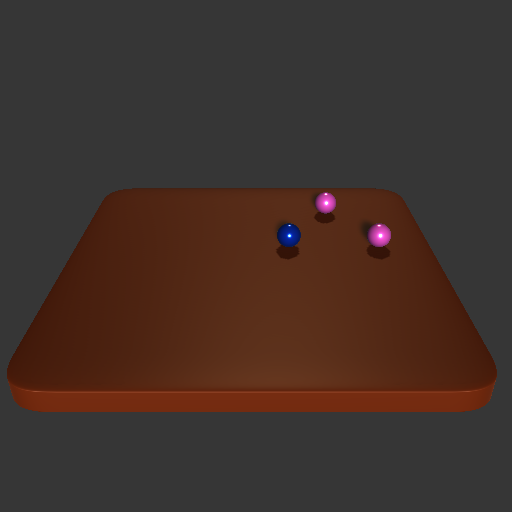
\includegraphics[width=0.24\textwidth]{img/hide/triangle_3.png}} 
	\subfigure[Vertical Line]{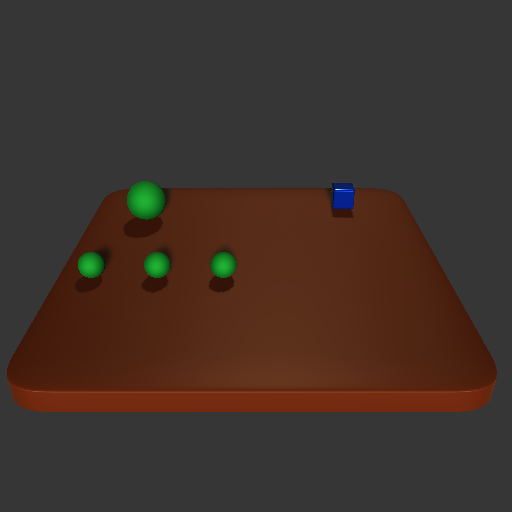
\includegraphics[width=0.24\textwidth]{img/hide/three_green_line.png}} 
	\subfigure[Pentagon]{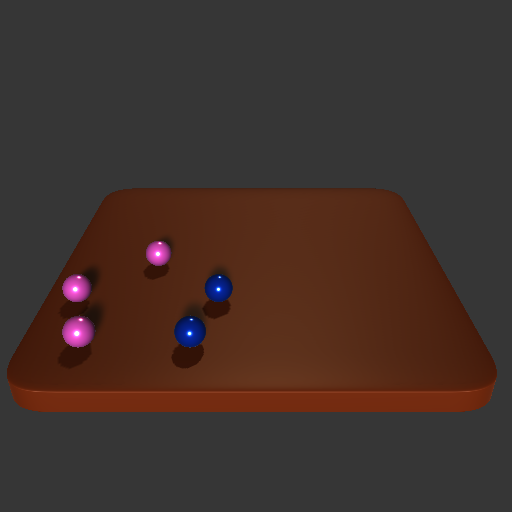
\includegraphics[width=0.24\textwidth]{img/hide/pentagon.png}}
	
	\subfigure[Triangle]{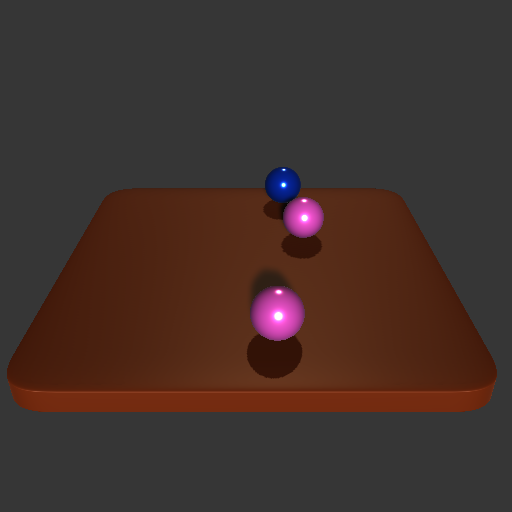
\includegraphics[width=0.24\textwidth]{img/hide/triangle_3_neg.png}} 
	\subfigure[Vertical Line]{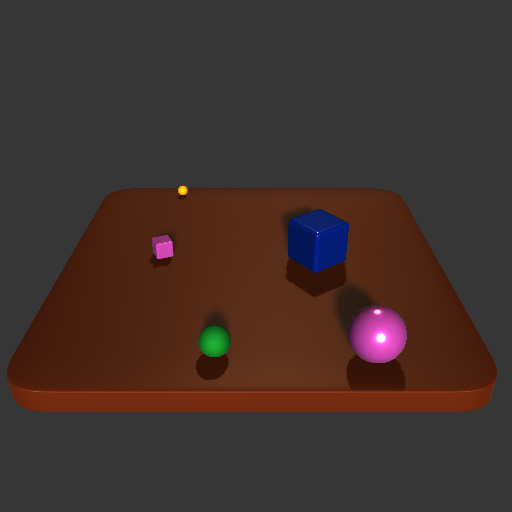
\includegraphics[width=0.24\textwidth]{img/hide/three_green_line_neg.png}} 
	\subfigure[Pentagon]{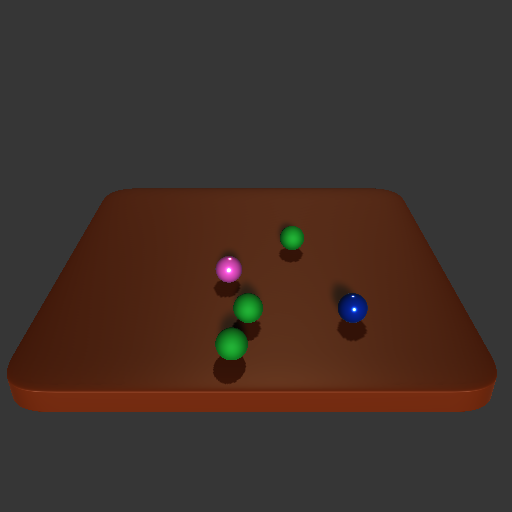
\includegraphics[width=0.24\textwidth]{img/hide/pentagon_neg.png}}
	\caption{Hide Patterns.}
	\label{fig:hide-patterns}
\end{figure}



\textbf{Necessary Condition}: % Invented predicates, on the contrary to the target predicate, should be \textit{necessary} for positive patterns. 
Necessary conditions can be entailed by all positive patterns. They can be insufficient, thus they can also be entailed by negative patterns. Necessary predicates are invented as prerequisite for sufficient predicate invention.
The necessity guarantees the searching for invented predicates is controlled in a proper scale, since only limited necessary conditions exist in the positive patterns. 
If we loose the necessity assumption, the searching domain for invented predicates can be huge since the conditions that doesn't exist in the positive patterns are irregular and  countless. 
In order to satisfy the necessary condition, we can \textbf{cluster} independent clauses. Independent means the clauses do not share same predicates. It usually leads to invent high level concepts. For example, cluster low level concept \textit{south}, \textit{east}, \textit{north}, \textit{west}, those are independent concept with each other, we can have a high level concept \textit{directions}. In this case, we need a new predicate to represent the cluster. Therefore the predicates are invented by necessary condition satisfied.



Think about "How" to cluster the existing clauses. Simply cluster all the clauses as one single concept cannot handle complicate rules.

If NSFR gives following clauses, then which of those clauses should be clustered as the new concept?

If there is a pattern with multiple rules,
a iteration-based approach should be proposed.
First several iteration, it should be able to learn some new predicates, then use new predicates to describe the new scenarios.

New predicate has to be able to 100\% describe the positive images. Otherwise, reconsider it.

\begin{align*}
	target(X,Y) &\leftarrow atArea0(X,Y), atArea2(Y,X)  \\
	target(X,Y) &\leftarrow atArea1(X,Y),atArea3(Y,X) \\
	target(X,Y) &\leftarrow atArea1(X,Y) \\    
	target(X,Y) &\leftarrow atArea2(X,Y) \\    
	target(X,Y) &\leftarrow atArea4(X,Y),atArea6(Y,X) \\
	target(X,Y) &\leftarrow atArea5(X,Y),atArea7(Y,X) \\
	target(X,Y) &\leftarrow atArea5(X,Y) \\    
	target(X,Y) &\leftarrow atArea6(X,Y) \\
	target(X,Y) &\leftarrow pred1(X,Y) \\
\end{align*}




\subsection{Chaining}
\cite{dILP} supports predicate invention.


\section{Experiments}

Using the baseline $\alpha$ILP, the nearby concept test accuracy is upto xxx, after xxx iterations.





\section{Modifications}

Modifying the template --- including but not limited to: adjusting
margins, typeface sizes, line spacing, paragraph and list definitions,
and the use of the \verb|\vspace| command to manually adjust the
vertical spacing between elements of your work --- is not allowed.

\section{Template parameters}

There are a number of template
parameters which modify some part of the \verb|ceurart| document class.
This parameters are enclosed in square
brackets and are a part of the \verb|\documentclass| command:
\begin{lstlisting}
  \documentclass[parameter]{ceurart}
\end{lstlisting}

Frequently-used parameters, or combinations of parameters, include:
\begin{itemize}
\item \verb|twocolumn| : Two column layout.
\item \verb|hf| : Enable header and footer\footnote{You can enable
    the display of page numbers in the final version of the entire
    collection. In this case, you should adhere to the end-to-end
    pagination of individual papers.}.
\end{itemize}

\section{Front matter}

\subsection{Title Information}

The titles of papers should be either all use the emphasizing
capitalized style or they should all use the regular English (or
native language) style. It does not make a good impression if you or
your authors mix the styles.

Use the \verb|\title| command to define the title of your work. Do not
insert line breaks in your title.

\subsection{Title variants}

\verb|\title| command have the below options:
\begin{itemize}
\item \verb|title|: Document title. This is default option. 
\begin{lstlisting}
\title[mode=title]{This is a title}
\end{lstlisting}
You can just omit it, like as follows:
\begin{lstlisting}
\title{This is a title}
\end{lstlisting}

\item \verb|alt|: Alternate title.
\begin{lstlisting}
\title[mode=alt]{This is a alternate title}
\end{lstlisting}

\item \verb|sub|: Sub title.
\begin{lstlisting}
\title[mode=sub]{This is a sub title}
\end{lstlisting}
You can just use \verb|\subtitle| command, as follows:
\begin{lstlisting}
\subtitle{This is a sub title}
\end{lstlisting}

\item \verb|trans|: Translated title.
\begin{lstlisting}
\title[mode=trans]{This is a translated title}
\end{lstlisting}

\item \verb|transsub|: Translated sub title.
\begin{lstlisting}
\title[mode=transsub]{This is a translated sub title}
\end{lstlisting}
\end{itemize}

\subsection{Authors and Affiliations}

Each author must be defined separately for accurate metadata
identification. Multiple authors may share one affiliation. Authors'
names should not be abbreviated; use full first names wherever
possible. Include authors' e-mail addresses whenever possible.

\verb|\author| command have the below options: 

\begin{itemize}
\item \verb|style| : Style of author name (chinese)
\item \verb|prefix| : Prefix
\item \verb|suffix| : Suffix
\item \verb|degree| : Degree
\item \verb|role| : Role
\item \verb|orcid| : ORCID
\item \verb|email| : E-mail
\item \verb|url| : URL
\end{itemize}

Author names can have some kinds of marks and notes:
\begin{itemize}
\item affiliation mark: \verb|\author[<num>]|.
\end{itemize}

The author names and affiliations could be formatted in two ways:
\begin{enumerate}
\item Group the authors per affiliation.
\item Use an explicit mark to indicate the affiliations.
\end{enumerate}

Author block example:
\begin{lstlisting}
\author[1,2]{Author Name}[%
    prefix=Prof.,
    degree=D.Sc.,
    role=Researcher,
    orcid=0000-0000-000-0000,
    email=name@example.com,
    url=https://name.example.com
]

\address[1]{Affiliation #1}
\address[2]{Affiliation #2}
\end{lstlisting}

\subsection{Abstract and Keywords}

Abstract shall be entered in an environment that starts
with \verb|\begin{abstract}| and ends with
\verb|\end{abstract}|. 

\begin{lstlisting}
\begin{abstract}
  This is an abstract.
\end{abstract}
\end{lstlisting}

The key words are enclosed in a \verb|keywords|
environment. Use \verb|\sep| to separate keywords.

\begin{lstlisting}
\begin{keywords}
  First keyword \sep 
  Second keyword \sep 
  Third keyword \sep 
  Fourth keyword
\end{keywords}
\end{lstlisting}

At the end of front matter add \verb|\maketitle| command.

\subsection{Various Marks in the Front Matter}

The front matter becomes complicated due to various kinds
of notes and marks to the title and author names. Marks in
the title will be denoted by a star ($\star$) mark;
footnotes are denoted by super scripted Arabic numerals,
corresponding author by an Conformal asterisk (*) mark.

\subsubsection{Title marks}

Title mark can be entered by the command, \verb|\tnotemark[<num>]|
and the corresponding text can be entered with the command
\verb|\tnotetext[<num>]{<text>}|. An example will be:

\begin{lstlisting}
\title{A better way to format your document for CEUR-WS}

\tnotemark[1]
\tnotetext[1]{You can use this document as the template for preparing your
  publication. We recommend using the latest version of the ceurart style.}
\end{lstlisting}

\verb|\tnotemark| and \verb|\tnotetext| can be anywhere in
the front matter, but should be before \verb|\maketitle| command.

\subsubsection{Author marks}

Author names can have some kinds of marks and notes:
\begin{itemize}
\item footnote mark : \verb|\fnmark[<num>]|
\item footnote text : \verb|\fntext[<num>]{<text>}|
\item corresponding author mark : \verb|\cormark[<num>]|
\item corresponding author text : \verb|\cortext[<num>]{<text>}|
\end{itemize}

\subsubsection{Other marks}

At times, authors want footnotes which leave no marks in
the author names. The note text shall be listed as part of
the front matter notes. Class files provides
\verb|\nonumnote| for this purpose. The usage
\begin{lstlisting}
\nonumnote{<text>}
\end{lstlisting}
and should be entered anywhere before the \verb|\maketitle|
command for this to take effect. 

\section{Sectioning Commands}

Your work should use standard \LaTeX{} sectioning commands:
\verb|\section|, \verb|\subsection|,
\verb|\subsubsection|, and
\verb|\paragraph|. They should be numbered; do not remove
the numbering from the commands.

Simulating a sectioning command by setting the first word or words of
a paragraph in boldface or italicized text is not allowed.

\section{Tables}

The ``\verb|ceurart|'' document class includes the ``\verb|booktabs|''
package --- \url{https://ctan.org/pkg/booktabs} --- for preparing
high-quality tables.

Table captions are placed \textit{above} the table.

Because tables cannot be split across pages, the best placement for
them is typically the top of the page nearest their initial cite.  To
ensure this proper ``floating'' placement of tables, use the
environment \verb|table| to enclose the table's contents and the
table caption. The contents of the table itself must go in the
\verb|tabular| environment, to be aligned properly in rows and
columns, with the desired horizontal and vertical rules.

Immediately following this sentence is the point at which
Table~\ref{tab:freq} is included in the input file; compare the
placement of the table here with the table in the printed output of
this document.

\begin{table*}
  \caption{Frequency of Special Characters}
  \label{tab:freq}
  \begin{tabular}{ccl}
    \toprule
    Non-English or Math&Frequency&Comments\\
    \midrule
    \O & 1 in 1,000& For Swedish names\\
    $\pi$ & 1 in 5& Common in math\\
    \$ & 4 in 5 & Used in business\\
    $\Psi^2_1$ & 1 in 40,000& Unexplained usage\\
  \bottomrule
\end{tabular}
\end{table*}

To set a wider table, which takes up the whole width of the page's
live area, use the environment \verb|table*| to enclose the table's
contents and the table caption.  As with a single-column table, this
wide table will ``float'' to a location deemed more
desirable. Immediately following this sentence is the point at which
Table~\ref{tab:commands} is included in the input file; again, it is
instructive to compare the placement of the table here with the table
in the printed output of this document.

\begin{table}
  \caption{Some Typical Commands}
  \label{tab:commands}
  \begin{tabular}{ccl}
    \toprule
    Command &A Number & Comments\\
    \midrule
    \texttt{{\char'134}author} & 100& Author \\
    \texttt{{\char'134}table}& 300 & For tables\\
    \texttt{{\char'134}table*}& 400& For wider tables\\
    \bottomrule
  \end{tabular}
\end{table}

\section{Math Equations}

You may want to display math equations in three distinct styles:
inline, numbered or non-numbered display.  Each of the three are
discussed in the next sections.

\subsection{Inline (In-text) Equations}

A formula that appears in the running text is called an inline or
in-text formula.  It is produced by the \verb|math| environment,
which can be invoked with the usual
\verb|\begin| \ldots \verb|\end| construction or with
the short form \verb|$| \ldots \verb|$|. You can use any of the symbols
and structures, from $\alpha$ to $\omega$, available in
\LaTeX~\cite{Lamport:LaTeX};
this section will simply show a few
examples of in-text equations in context. Notice how this equation:
\begin{math}
  \lim_{n\rightarrow \infty} \frac{1}{n} = 0,
\end{math}
set here in in-line math style, looks slightly different when
set in display style.  (See next section).

\subsection{Display Equations}

A numbered display equation---one set off by vertical space from the
text and centered horizontally---is produced by the \verb|equation|
environment. An unnumbered display equation is produced by the
\verb|displaymath| environment.

Again, in either environment, you can use any of the symbols and
structures available in \LaTeX{}; this section will just give a couple
of examples of display equations in context.  First, consider the
equation, shown as an inline equation above:
\begin{equation}
  \lim_{n\rightarrow \infty} \frac{1}{n} = 0.
\end{equation}
Notice how it is formatted somewhat differently in
the \verb|displaymath|
environment.  Now, we'll enter an unnumbered equation:
\begin{displaymath}
  S_{n} = \sum_{i=1}^{n} x_{i} ,
\end{displaymath}
and follow it with another numbered equation:
\begin{equation}
  \lim_{x \to 0} (1 + x)^{1/x} = e
\end{equation}
just to demonstrate \LaTeX's able handling of numbering.

\section{Figures}

The ``\verb|figure|'' environment should be used for figures. One or
more images can be placed within a figure. If your figure contains
third-party material, you must clearly identify it as such, as shown
in the example below.
\begin{figure}
  \centering
  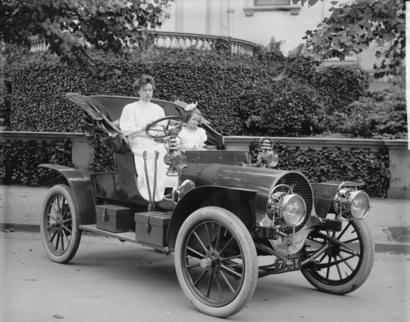
\includegraphics[width=\linewidth]{sample-franklin}
  \caption{1907 Franklin Model D roadster. Photograph by Harris \&
    Ewing, Inc. [Public domain], via Wikimedia
    Commons. (\url{https://goo.gl/VLCRBB}).}
\end{figure}

Your figures should contain a caption which describes the figure to
the reader. Figure captions go below the figure. Your figures should
also include a description suitable for screen readers, to
assist the visually-challenged to better understand your work.

Figure captions are placed below the figure.


\section{Introduction}

CEUR-WS's article template provides a consistent \LaTeX{} style for
use across CEUR-WS publications, and incorporates accessibility and
metadata-extraction functionality. This document will explain the
major features of the document class.

If you are new to publishing with CEUR-WS, this document is a valuable
guide to the process of preparing your work for publication.

The ``\verb|ceurart|'' document class can be used to prepare articles
for any CEUR-WS publication, and for any stage of publication, from
review to final ``camera-ready'' copy with {\itshape very} few changes
to the source.

This class depends on the following packages
for its proper functioning:

\begin{itemize}
	\item \verb|natbib.sty| for citation processing;
	\item \verb|geometry.sty| for margin settings;
	\item \verb|graphicx.sty| for graphics inclusion;
	\item \verb|hyperref.sty| optional package if hyperlinking is required in
	the document;
	\item \verb|fontawesome5.sty| optional package for bells and whistles.
\end{itemize}

All the above packages are part of any
standard \LaTeX{} installation.
Therefore, the users need not be
bothered about downloading any extra packages.



\section{Citations and Bibliographies}

The use of Bib\TeX{} for the preparation and formatting of one's
references is strongly recommended. Authors' names should be complete
--- use full first names (``Donald E. Knuth'') not initials
(``D. E. Knuth'') --- and the salient identifying features of a
reference should be included: title, year, volume, number, pages,
article DOI, etc.

The bibliography is included in your source document with these two
commands, placed just before the \verb|\end{document}|
command:
\begin{lstlisting}
\bibliography{bibfile}
\end{lstlisting}
where ``\verb|bibfile|'' is the name, without the ``\verb|.bib|''
suffix, of the Bib\TeX{} file.


\subsection{Some examples}

A paginated journal article \cite{Abril07}, an enumerated journal
article \cite{Cohen07}, a reference to an entire issue
\cite{JCohen96}, a monograph (whole book) \cite{Kosiur01}, a
monograph/whole book in a series (see 2a in spec. document)
\cite{Harel79}, a divisible-book such as an anthology or compilation
\cite{Editor00} followed by the same example, however we only output
the series if the volume number is given \cite{Editor00a} (so series
should not be present since it has no vol. no.), a chapter in a
divisible book \cite{Spector90}, a chapter in a divisible book in a
series \cite{Douglass98}, a multi-volume work as book \cite{Knuth97},
an article in a proceedings (of a conference, symposium, workshop for
example) (paginated proceedings article) \cite{Andler79}, a
proceedings article with all possible elements \cite{Smith10}, an
example of an enumerated proceedings article \cite{VanGundy07}, an
informally published work \cite{Harel78}, a doctoral dissertation
\cite{Clarkson85}, a master's thesis: \cite{anisi03}, an online
document / world wide web resource \cite{Thornburg01, Ablamowicz07,
  Poker06}, a video game (Case 1) \cite{Obama08} and (Case 2)
\cite{Novak03} and \cite{Lee05} and (Case 3) a patent
\cite{JoeScientist001}, work accepted for publication \cite{rous08},
prolific author \cite{SaeediMEJ10} and \cite{SaeediJETC10}. Other
cites might contain `duplicate' DOI and URLs (some SIAM articles)
\cite{Kirschmer:2010:AEI:1958016.1958018}. Multi-volume works as books
\cite{MR781536} and \cite{MR781537}. A couple of citations with DOIs:
\cite{2004:ITE:1009386.1010128,Kirschmer:2010:AEI:1958016.1958018}. Online
citations: \cite{TUGInstmem, Thornburg01, R, UMassCitations}.

\section{Acknowledgments}

Identification of funding sources and other support, and thanks to
individuals and groups that assisted in the research and the
preparation of the work should be included in an acknowledgment
section, which is placed just before the reference section in your
document.

This section has a special environment:
\begin{lstlisting}
\begin{acknowledgments}
  These are different acknowledgments.
\end{acknowledgments}
\end{lstlisting}
so that the information contained therein can be more easily collected
during the article metadata extraction phase, and to ensure
consistency in the spelling of the section heading.

Authors should not prepare this section as a numbered or unnumbered
\verb|\section|; please use the ``\verb|acknowledgments|'' environment.

\section{Appendices}

If your work needs an appendix, add it before the
``\verb|\end{document}|'' command at the conclusion of your source
document.

Start the appendix with the ``\verb|\appendix|'' command:
\begin{lstlisting}
\appendix
\end{lstlisting}
and note that in the appendix, sections are lettered, not
numbered. 

%%
%% The acknowledgments section is defined using the "acknowledgments" environment
%% (and NOT an unnumbered section). This ensures the proper
%% identification of the section in the article metadata, and the
%% consistent spelling of the heading.
\begin{acknowledgments}
  Thanks to the developers of ACM consolidated LaTeX styles
  \url{https://github.com/borisveytsman/acmart} and to the developers
  of Elsevier updated \LaTeX{} templates
  \url{https://www.ctan.org/tex-archive/macros/latex/contrib/els-cas-templates}.  
\end{acknowledgments}

%%
%% Define the bibliography file to be used
\bibliography{sample-ceur}

%%
%% If your work has an appendix, this is the place to put it.
\appendix

\section{Online Resources}


The sources for the ceur-art style are available via
\begin{itemize}
\item \href{https://github.com/yamadharma/ceurart}{GitHub},
% \item \href{https://www.overleaf.com/project/5e76702c4acae70001d3bc87}{Overleaf},
\item
  \href{https://www.overleaf.com/latex/templates/template-for-submissions-to-ceur-workshop-proceedings-ceur-ws-dot-org/pkfscdkgkhcq}{Overleaf
    template}.
\end{itemize}

\end{document}

%%
%% End of file
